\section{Methodology}
\label{sec:method}
% include the figures path relative to the master file
\graphicspath{ {./content/method/figures/} }

% \begin{figure}[t]
%     \centering
%     \begin{subfigure}[b]{0.30\textwidth}
%         \centering
%         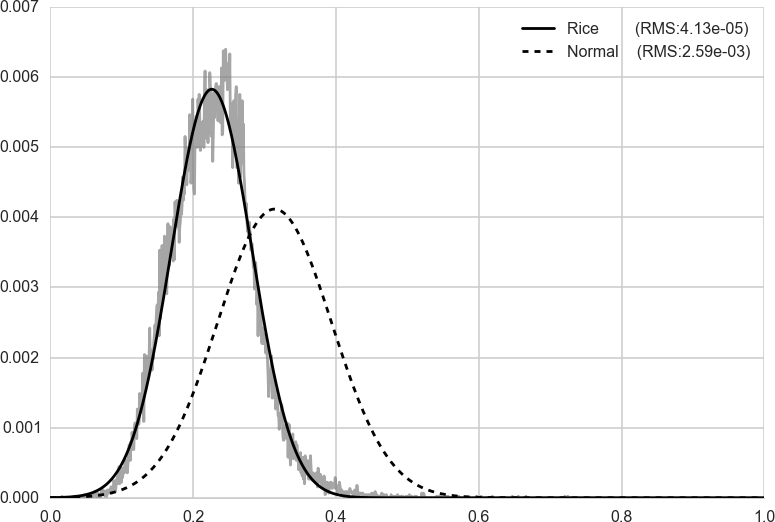
\includegraphics[width=\textwidth]{03}
%     \end{subfigure}
%     \hfill
%     \begin{subfigure}[b]{0.30\textwidth}
%         \centering
%         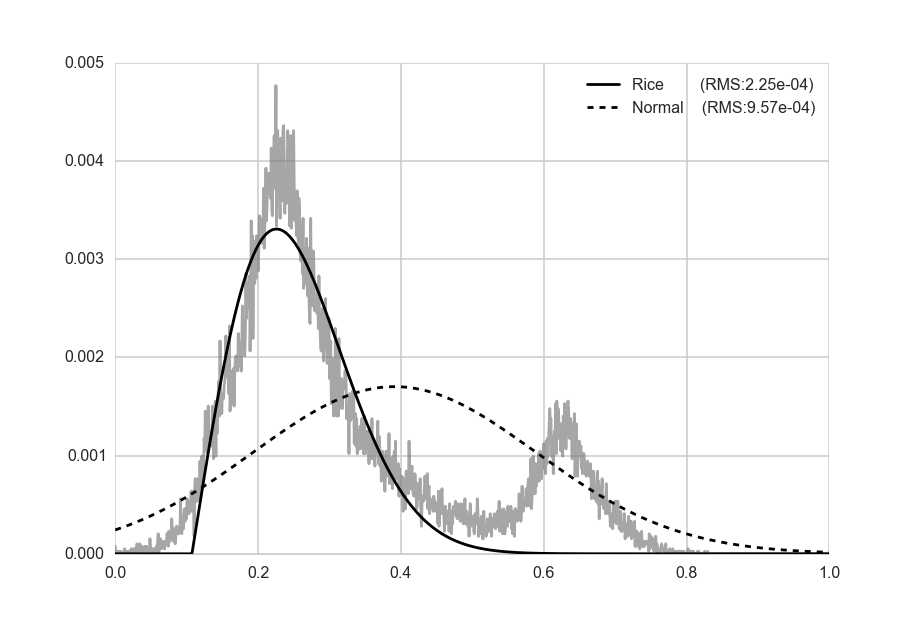
\includegraphics[width=\textwidth]{06}
%     \end{subfigure}
%     \hfill
%     \begin{subfigure}[b]{0.30\textwidth}
%         \centering
%         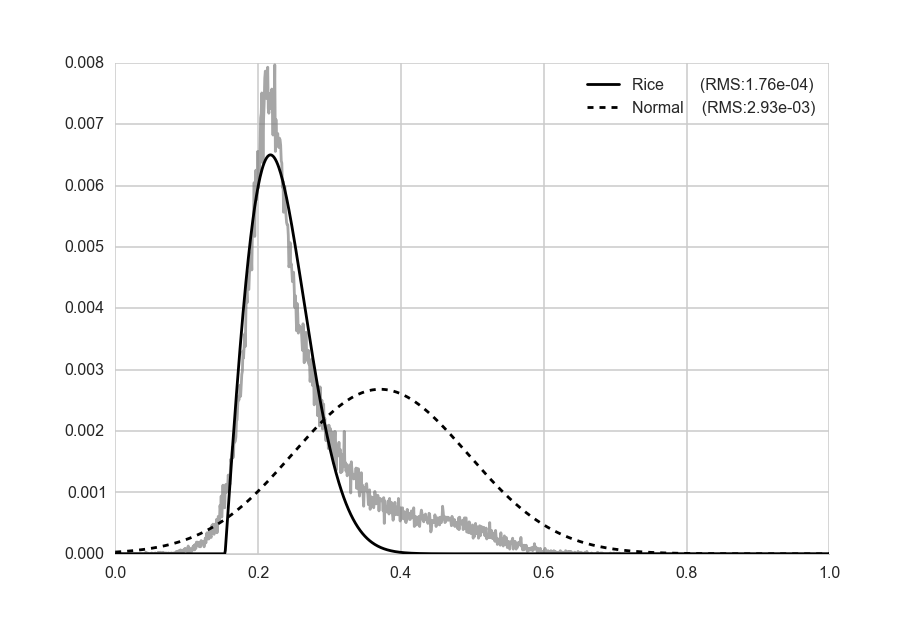
\includegraphics[width=\textwidth]{14}
%     \end{subfigure}
%     \caption {Fitting differences}
%     \label{fig:rice-norm-diff}
% \end{figure}

\subsection{Normalization using Rician \textit{a priori}}

As stated in~Sect.\,\ref{sec:intro}, proper normalization of the \ac{mri} data during pre-processing is a key problem that has been addressed using parametric and non-parametric strategies.
We believe that normalizing \ac{mri} data using a parametric model based on a Rician distribution would improve the results for the parametric case.
Expecting this improvement by changing the data model from the widely used Gaussian distribution to Rician distribution is reasonable. 
Indeed, Bernstein\,\textit{et al.}~\cite{bernstein1989improved} state that \ac{mri} data theoretically follows a Rayleigh distribution for a low \ac{snr} scenarios while it appears closer to a Gaussian distribution when the \ac{snr} increases.
Figure~\ref{fig:fitting} shows the intensity spectrum for some \ac{mri} prostate data as well as the fitted Gaussian and Rician distributions.
A qualitative assessment of the underlying distribution is performed by overlying the fitted distribution, while quantitative results of the fitting are given in terms of \ac{rms}.
It can be highlighted that the Rician model better fits the data than the Gaussian model.

\begin{figure*}
  \centering
  \subfloat[][]{
    \label{fig:p1}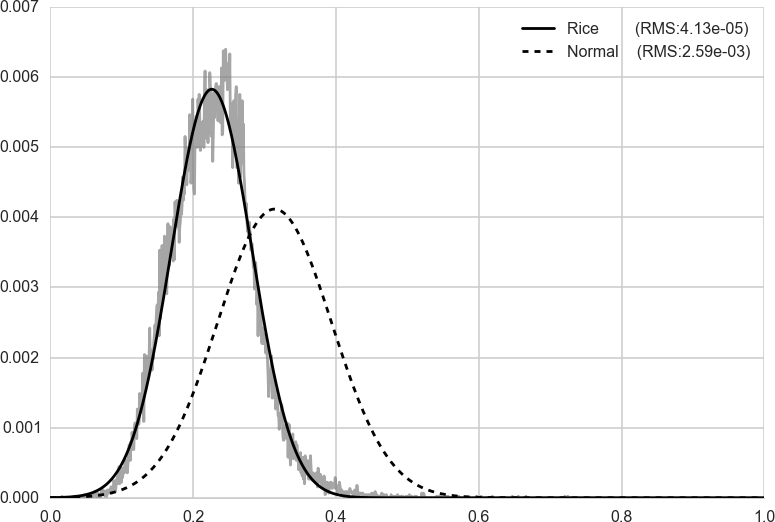
\includegraphics[width=0.25\textwidth]{03}}\hfill
  \subfloat[][]{
    \label{fig:p2}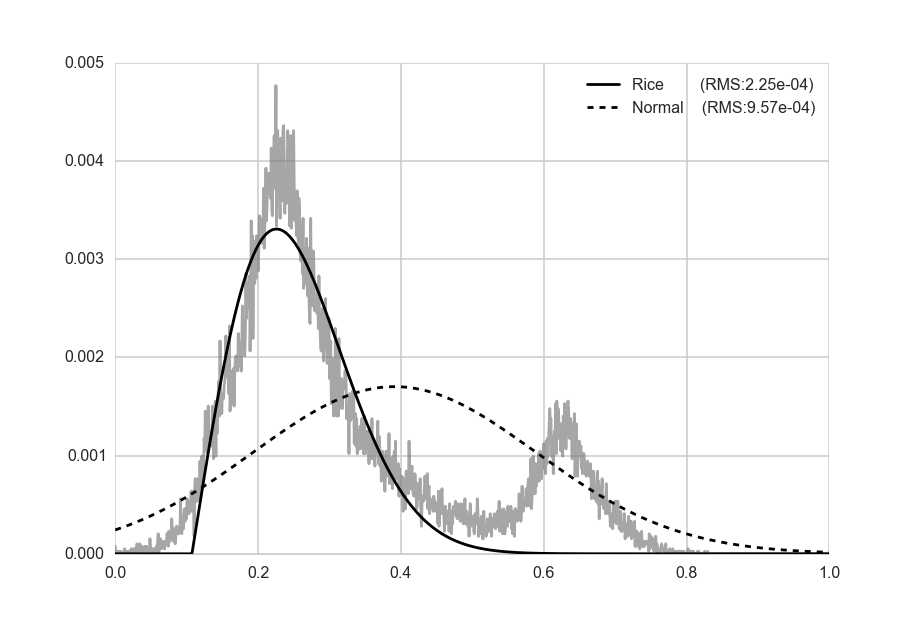
\includegraphics[width=0.25\textwidth]{06}}\hfill
  \subfloat[][]{
    \label{fig:p3}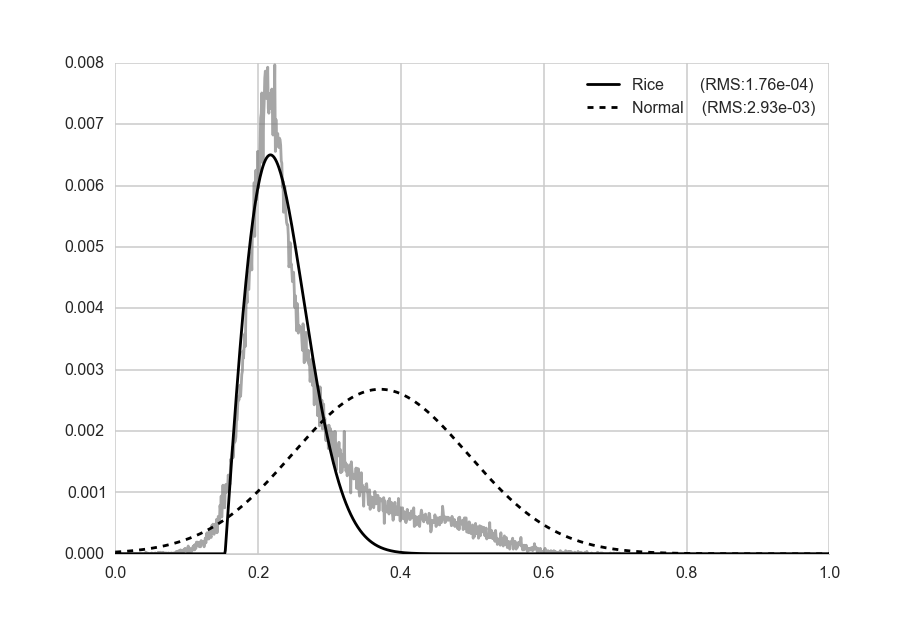
\includegraphics[width=0.25\textwidth]{14}}
  \caption{Visual evaluation of the goodness of fitting using Rician and Gaussian distribution.}
  \label{fig:fitting}
\end{figure*}

The normalization is carried out as: 
(i) Fit a Rician model to each prostate \ac{pdf} using Least Squares minimization; 
(ii) Compute the mean (see~Eq.\,\eqref{eq:mean}) and variance (see~Eq.\,\eqref{eq:var}) of the Rician model;
(iii) Normalize the entire data using the \textit{z-score} similarly as in~Eq.\,\eqref{eq:zscore}.

\begin{equation}
  \sigma  \sqrt{\pi/2}\,\,L_{1/2}(-\nu^2/2\sigma^2) 
  \label{eq:mean}
\end{equation}
\vspace{-.4cm}
\begin{equation}
  2\sigma^2+\nu^2-\frac{\pi\sigma^2}{2}L_{1/2}^2\left(\frac{-\nu^2}{2\sigma^2}\right) 
  \label{eq:var}
\end{equation}

\subsection{Normalization using generative models in functional data analysis}


%%% Local Variables: 
%%% mode: latex
%%% TeX-master: "../../master"
%%% End: 

